
\documentclass[11pt,a4paper]{article}

%============================================================

% ------------------------------------------------------------
% Packages
% ------------------------------------------------------------
\usepackage[a4paper,margin=21mm]{geometry}
\usepackage[T1]{fontenc}
\usepackage[utf8]{inputenc}
\usepackage{lmodern}
\usepackage{microtype}
\usepackage{amsmath,amssymb}
\usepackage{siunitx}
\usepackage{booktabs}
\usepackage{array}
\usepackage{tabularx}
\usepackage{longtable}
\usepackage{multirow}
\usepackage{graphicx}
\usepackage{float}
\usepackage[american]{circuitikz}
\usepackage{pgfplots}
\pgfplotsset{compat=1.18}
\usepackage{xcolor}
\usepackage[most]{tcolorbox}
\usepackage{enumitem}
\usepackage{fancyhdr}
\usepackage{hyperref}
\usepackage{caption}
\usepackage{lastpage}

% ------------------------------------------------------------
% Formatting
% ------------------------------------------------------------
\definecolor{cetblue}{RGB}{0,72,120}
\definecolor{lightblue}{RGB}{239,247,252}
\definecolor{lightgray}{RGB}{247,247,247}
\definecolor{lightyellow}{RGB}{255,249,225}
\definecolor{lightgreen}{RGB}{239,250,242}
\definecolor{lightred}{RGB}{255,242,242}

\hypersetup{
  colorlinks=true,
  linkcolor=cetblue,
  urlcolor=cetblue,
  citecolor=cetblue
}

\pagestyle{fancy}
\fancyhf{}
\lhead{Analog Circuits Lab}
\rhead{RC-Coupled BJT Amplifier}
\cfoot{Page \thepage\ of \pageref{LastPage}}
\setlength{\headheight}{14pt}

\setlist[itemize]{leftmargin=1.5em,itemsep=2pt,topsep=3pt}
\setlist[enumerate]{leftmargin=1.7em,itemsep=2pt,topsep=3pt}
\sisetup{
  per-mode=symbol,
  detect-all,
  group-separator={,},
  group-minimum-digits=4
}

\renewcommand{\arraystretch}{1.25}
\setlength{\parindent}{0pt}
\setlength{\parskip}{4pt}

% ------------------------------------------------------------
% Reusable boxes
% ------------------------------------------------------------
\newtcolorbox{sectionguide}{
  colback=lightblue,
  colframe=cetblue,
  boxrule=0.6pt,
  arc=2mm,
  title=What the student should include,
  fonttitle=\bfseries,
  left=2mm,right=2mm,top=1mm,bottom=1mm
}

\newtcolorbox{examplebox}{
  colback=lightgray,
  colframe=black!45,
  boxrule=0.5pt,
  arc=2mm,
  title=Illustrative example: RC-coupled BJT amplifier,
  fonttitle=\bfseries,
  left=2mm,right=2mm,top=1mm,bottom=1mm
}

\newtcolorbox{prelabbox}{
  colback=lightyellow,
  colframe=orange!75!black,
  boxrule=0.6pt,
  arc=2mm,
  title=Pre-lab requirement,
  fonttitle=\bfseries,
  left=2mm,right=2mm,top=1mm,bottom=1mm
}

\newtcolorbox{safetybox}{
  colback=lightred,
  colframe=red!65!black,
  boxrule=0.6pt,
  arc=2mm,
  title=Laboratory safety and conduct,
  fonttitle=\bfseries,
  left=2mm,right=2mm,top=1mm,bottom=1mm
}

\newtcolorbox{verificationbox}{
  colback=lightgreen,
  colframe=green!45!black,
  boxrule=0.6pt,
  arc=2mm,
  title=Instructor verification,
  fonttitle=\bfseries,
  left=2mm,right=2mm,top=1mm,bottom=1mm
}

\newcommand{\blankfield}[1]{\rule{#1}{0.4pt}}
\newcommand{\pcterror}{\%\,\text{error}}

\begin{document}

% ============================================================
% Compact report heading -- intentionally not a separate page
% ============================================================
\begin{center}
  {\LARGE\bfseries ANALOG CIRCUITS LAB}\\[1.5mm]
  {\large Third Semester -- Electronics and Communication Engineering}\\[1mm]
  {\large\bfseries College of Engineering Trivandrum}\\[3mm]
  {\Large\bfseries Laboratory Experiment Report}
\end{center}

\vspace{2mm}

\begin{tabularx}{\textwidth}{>{\bfseries}p{36mm} X >{\bfseries}p{36mm} X}
Experiment No. & 05 & Date of Experiment & \hrulefill \\
\end{tabularx}

\begin{tabularx}{\textwidth}{>{\bfseries}p{36mm} X}
Experiment Title & Design and Setup of an RC-Coupled Common-Emitter Amplifier Using a BJT \\
\end{tabularx}

\begin{tabularx}{\textwidth}{>{\bfseries}p{36mm} X >{\bfseries}p{36mm} X}
Student Name & \hrulefill & Roll No. & \hrulefill \\
University Reg. No. & \hrulefill & Batch / Group & \hrulefill \\
Team Member(s) & \multicolumn{3}{X}{\hrulefill} \\
Course Instructor & \hrulefill & Lab Instructor / TA & \hrulefill \\
Time of Experiment & \hrulefill & Laboratory / Workstation & \hrulefill \\
Date of Submission & \hrulefill & Student Signature & \hrulefill \\
\end{tabularx}

\vspace{3mm}
\hrule
\vspace{4mm}

% ============================================================
% Challenge-driven framing from the reference laboratory manual
% ============================================================
\begin{tcolorbox}[
  colback=white,
  colframe=cetblue,
  title=\textbf{Engineering Challenge and Deliverables},
  boxrule=0.7pt,
  arc=2mm
]
\textbf{Challenge statement:}
Design, simulate, construct, and evaluate a single-stage RC-coupled
common-emitter BJT amplifier that operates in the active region and provides
stable voltage amplification over a specified frequency range.

\textbf{Example design requirements:}
\begin{itemize}
  \item DC supply: $V_{CC}=\SI{12}{\volt}$.
  \item Quiescent collector-emitter voltage near the middle of the available
        output-swing range.
  \item Midband voltage gain magnitude greater than \SI{60}{\volt\per\volt}.
  \item Lower cutoff frequency below \SI{100}{\hertz}.
  \item Undistorted sinusoidal output for the prescribed small input signal.
\end{itemize}

\textbf{Required deliverables:}
completed pre-lab design, simulation, neat circuit schematic, verified
instrument and component list, recorded raw measurements, calculations,
frequency-response graph, theory--simulation--measurement comparison,
uncertainty/error analysis, conclusion, and an individually written report.
\end{tcolorbox}

\begin{prelabbox}
The student should read the complete experiment, review the relevant theory,
finish the required calculations and simulation, predict the expected
waveforms, and prepare observation tables \emph{before} entering the
laboratory. The pre-lab is part of the engineering design process, not an
optional preliminary exercise.
\end{prelabbox}

\begin{safetybox}
Switch off the DC supply before inserting, removing, or rewiring components.
Set a suitable current limit before energising the circuit. Verify transistor
pin configuration and electrolytic-capacitor polarity. Never measure
resistance in an energised circuit. Use a common ground correctly, avoid
shorting the supply through oscilloscope ground leads, and return instruments,
components, and leads to their designated locations after the experiment.
\end{safetybox}

% ============================================================
\section{Objective}
% ============================================================
\begin{sectionguide}
\begin{itemize}
  \item State the purpose in measurable engineering terms.
  \item Identify the circuit topology and the quantities to be designed,
        measured, and compared.
  \item Relate the objectives to the challenge specifications.
  \item Avoid vague wording such as ``to study the amplifier.''
\end{itemize}
\end{sectionguide}

\begin{examplebox}
The objectives of the experiment are:
\begin{enumerate}
  \item To design and construct a single-stage RC-coupled common-emitter
        amplifier using an NPN BJT.
  \item To establish a stable DC operating point that permits approximately
        symmetrical output-voltage swing.
  \item To simulate and experimentally determine the midband voltage gain,
        lower cutoff frequency, upper cutoff frequency, and bandwidth.
  \item To observe the approximately $180^\circ$ phase reversal between
        input and output.
  \item To compare theoretical, simulated, and experimental values and
        explain the important differences using component tolerance,
        transistor variation, loading, and parasitic effects.
\end{enumerate}
\end{examplebox}

% ============================================================
\section{Background Theory}
% ============================================================
\begin{sectionguide}
\begin{itemize}
  \item Establish the scientific and engineering context of the experiment.
  \item Explain the operation of the common-emitter amplifier and the purpose
        of each resistor and capacitor.
  \item Present only the equations needed for design and interpretation.
  \item State assumptions, including active-region operation, small-signal
        excitation, room temperature, and nominal transistor current gain.
  \item Include a clear prediction or design hypothesis that will later be
        tested by the measurements.
  \item Cite the textbook, laboratory manual, datasheet, or other sources used.
\end{itemize}
\end{sectionguide}

\begin{examplebox}
A common-emitter amplifier produces voltage gain and an output that is
approximately $180^\circ$ out of phase with its input. The voltage-divider
network $R_1$--$R_2$ biases the transistor base. The emitter resistor $R_E$
improves thermal and bias stability, while $R_C$ converts changes in collector
current into changes in collector voltage.

The coupling capacitors $C_1$ and $C_2$ pass the AC signal while isolating the
DC bias of the amplifier from the source and load. The emitter-bypass
capacitor $C_E$ provides a low-reactance AC path around $R_E$ in the intended
frequency band, thereby increasing AC gain without removing DC stabilisation.

For a transistor operating in its active region,
\begin{align}
I_C &\approx \beta I_B,\\
I_E &\approx (\beta+1)I_B,\\
V_{CE} &= V_C-V_E .
\end{align}

The intrinsic small-signal emitter resistance is approximately
\begin{equation}
r_e \approx \frac{V_T}{I_E},
\end{equation}
where $V_T\approx\SI{25}{\milli\volt}$ at room temperature. When $R_E$ is
effectively bypassed at midband, an approximate stage gain is
\begin{equation}
A_v \approx -\frac{R_C\parallel R_L}{r_e+X_{C_E,\mathrm{effective}}}.
\end{equation}
A more accurate prediction should also include source loading, finite
transistor current gain, transistor output resistance, and the bias network.

The lower cutoff frequency is governed mainly by $C_1$, $C_2$, and $C_E$.
The upper cutoff frequency is governed mainly by transistor junction
capacitances, the Miller effect, wiring capacitance, and probe loading.
The bandwidth is
\begin{equation}
BW=f_H-f_L.
\end{equation}

\textbf{Design hypothesis:}
If the transistor is biased near the middle of its usable output-swing range
and the capacitors are selected so that their reactances are sufficiently
small in the midband, the constructed circuit will provide a nearly constant
midband gain greater than \SI{60}{\volt\per\volt}, with reduced gain below
$f_L$ and above $f_H$.
\end{examplebox}

% ============================================================
\section{Circuit Diagram}
% ============================================================
\begin{sectionguide}
\begin{itemize}
  \item Draw a neat schematic showing correct interconnections.
  \item Label the transistor, all component reference names and values,
        $V_{CC}$, input, output, and ground.
  \item Mark important measurement nodes: base, collector, and emitter.
  \item Show the source resistance and external load when they affect results.
  \item Ensure the final schematic represents the circuit actually built;
        document any in-lab component substitution.
\end{itemize}
\end{sectionguide}

\begin{figure}[H]
\centering
\begin{circuitikz}[american voltages, scale=0.93, transform shape]
  % Signal source and input coupling
  \draw
  (0,0) node[ground]{}
  to[sV,l_=$v_s$] (0,2)
  to[R,l=$R_s$] (2,2)
  to[C,l=$C_1$] (4,2) coordinate(B);

  % Bias network
  \draw (B) to[R,l_=$R_2$] (4,0) node[ground]{};
  \draw (B) to[R,l=$R_1$] (4,4) -- (6,4) node[vcc]{$V_{CC}$};

  % BJT
  \node[npn, anchor=B] (Q1) at (5.7,2) {};
  \node[right] at (Q1) {$Q_1$};
  \draw (B) -- (Q1.B);

  % Collector
  \draw (Q1.C) to[R,l=$R_C$] (5.7,4) -- (6,4);

  % Emitter and bypass
  \draw (Q1.E) to[R,l=$R_E$] (5.7,0) node[ground]{};
  \draw (Q1.E) -- (7.2,1.2)
        to[C,l=$C_E$] (7.2,0) node[ground]{};

  % Output
  \draw (Q1.C) -- (7.0,2.8)
        to[C,l=$C_2$] (8.6,2.8) coordinate(OUT);
  \draw (OUT) to[R,l=$R_L$] (8.6,0) node[ground]{};
  \draw (OUT) to[short,-o] (9.7,2.8) node[right]{$v_o$};

  % Labels
  \node[above left] at (Q1.B) {$V_B$};
  \node[above right] at (Q1.C) {$V_C$};
  \node[below right] at (Q1.E) {$V_E$};
\end{circuitikz}
\caption{Single-stage RC-coupled common-emitter BJT amplifier.}
\label{fig:circuit}
\end{figure}

\begin{examplebox}
\begin{center}
\begin{tabular}{lll}
\toprule
Item & Nominal value / type & Function \\
\midrule
$Q_1$ & BC547B & NPN amplifying device \\
$V_{CC}$ & \SI{12}{\volt} & DC supply \\
$R_1$ & \SI{100}{\kilo\ohm} & Upper bias resistor \\
$R_2$ & \SI{18}{\kilo\ohm} & Lower bias resistor \\
$R_C$ & \SI{4.7}{\kilo\ohm} & Collector resistor \\
$R_E$ & \SI{1}{\kilo\ohm} & DC stabilisation resistor \\
$C_1$ & \SI{1}{\micro\farad} & Input coupling capacitor \\
$C_2$ & \SI{1}{\micro\farad} & Output coupling capacitor \\
$C_E$ & \SI{47}{\micro\farad} & Emitter bypass capacitor \\
$R_L$ & \SI{10}{\kilo\ohm} & External load \\
$R_s$ & \SI{600}{\ohm} & Representative source resistance \\
\bottomrule
\end{tabular}
\end{center}
\end{examplebox}

% ============================================================
\section{Equipment and Software Required}
% ============================================================
\begin{sectionguide}
\begin{itemize}
  \item Specify every test instrument using manufacturer and model/type number.
  \item Record relevant instrument settings or specifications such as
        bandwidth, input impedance, probe attenuation, and source impedance.
  \item List component type, nominal value, measured value, tolerance, and
        power or voltage rating where relevant.
  \item Identify the simulator, software version, transistor model/library,
        and analyses performed.
  \item List breadboard, probes, BNC leads, connecting wires, and other
        materials required for reproducibility.
\end{itemize}
\end{sectionguide}

\begin{examplebox}
\textbf{Illustrative equipment list:}
\begin{itemize}
  \item Regulated DC power supply, \SIrange{0}{30}{\volt}, with current-limit
        facility; manufacturer/model: \underline{\hspace{50mm}}.
  \item Dual-channel digital storage oscilloscope, minimum
        \SI{20}{\mega\hertz} bandwidth; manufacturer/model:
        \underline{\hspace{42mm}}.
  \item Function generator with sine-wave output; manufacturer/model:
        \underline{\hspace{44mm}}.
  \item Digital multimeter; manufacturer/model:
        \underline{\hspace{59mm}}.
  \item Two $10\times$ oscilloscope probes, breadboard, BNC leads, and
        connecting wires.
  \item BC547B NPN transistor, resistors, and capacitors listed with
        Figure~\ref{fig:circuit}.
  \item LTspice / PSpice / Multisim, version:
        \underline{\hspace{35mm}}; transistor model:
        \underline{\hspace{35mm}}.
\end{itemize}

\textbf{Component-verification table:}
\begin{center}
\begin{tabular}{lcccc}
\toprule
Component & Nominal & Measured & Tolerance/rating & Used value \\
\midrule
$R_1$ & \SI{100}{\kilo\ohm} & \SI{98.7}{\kilo\ohm} & $\pm5\%$ & \SI{98.7}{\kilo\ohm} \\
$R_2$ & \SI{18}{\kilo\ohm} & \SI{17.9}{\kilo\ohm} & $\pm5\%$ & \SI{17.9}{\kilo\ohm} \\
$R_C$ & \SI{4.7}{\kilo\ohm} & \SI{4.66}{\kilo\ohm} & $\pm5\%$ & \SI{4.66}{\kilo\ohm} \\
$R_E$ & \SI{1}{\kilo\ohm} & \SI{0.99}{\kilo\ohm} & $\pm5\%$ & \SI{0.99}{\kilo\ohm} \\
$C_E$ & \SI{47}{\micro\farad} & --- & \SI{25}{\volt}, $\pm20\%$ & \SI{47}{\micro\farad} \\
\bottomrule
\end{tabular}
\end{center}
\end{examplebox}

% ============================================================
\section{Pre-Lab Calculations and Design}
% ============================================================
\begin{sectionguide}
\begin{itemize}
  \item Record initial thoughts on how the challenge can be solved.
  \item State design specifications, assumptions, and the proposed topology.
  \item Complete DC bias design, small-signal analysis, capacitor selection,
        predicted gain, output swing, and cutoff-frequency calculations.
  \item Use standard component values and then recompute expected performance.
  \item Prepare expected waveforms and an expected frequency-response sketch.
  \item Perform and document DC operating-point, AC sweep, and transient
        simulations before construction.
  \item Identify risks and checks: transistor pinout, clipping, saturation,
        capacitor polarity, and maximum device ratings.
\end{itemize}
\end{sectionguide}

\subsection*{6.1 Initial thoughts and proposed solution}

\begin{examplebox}
A voltage-divider-biased common-emitter stage was selected because it provides
higher bias stability than fixed bias. An emitter resistor was retained for DC
negative feedback, while a bypass capacitor was added to obtain higher AC
gain. The collector voltage was targeted near the middle of the supply range
to allow approximately symmetrical output swing. Input and output coupling
capacitors were used to prevent the source and load from disturbing the DC
bias.

The design was expected to meet the gain requirement if the transistor
remained in the active region and the emitter bypass capacitor presented
sufficiently low reactance in the intended midband.
\end{examplebox}

\subsection*{6.2 DC bias design}

\begin{examplebox}
Assume
\[
V_{CC}=\SI{12}{\volt},\qquad
\beta=100,\qquad
V_{BE}=\SI{0.7}{\volt},\qquad
R_E=\SI{1}{\kilo\ohm}.
\]

For $R_1=\SI{100}{\kilo\ohm}$ and
$R_2=\SI{18}{\kilo\ohm}$, the Thevenin equivalent at the base is
\begin{align}
V_{TH}
 &=V_{CC}\frac{R_2}{R_1+R_2}
 =12\frac{18}{100+18}
 =\SI{1.83}{\volt},\\
R_{TH}
 &=R_1\parallel R_2
 =\SI{15.25}{\kilo\ohm}.
\end{align}

The base current is estimated as
\begin{equation}
I_B=
\frac{V_{TH}-V_{BE}}{R_{TH}+(\beta+1)R_E}
=
\frac{1.83-0.70}
{15.25\,\text{k}+101(1\,\text{k})}
\approx\SI{9.72}{\micro\ampere}.
\end{equation}

Therefore,
\begin{align}
I_C &\approx \beta I_B=\SI{0.972}{\milli\ampere},\\
I_E &\approx(\beta+1)I_B=\SI{0.982}{\milli\ampere},\\
V_E &=I_E R_E\approx\SI{0.982}{\volt},\\
V_C &=V_{CC}-I_C R_C
    \approx 12-(0.972\,\text{m})(4.7\,\text{k})
    =\SI{7.43}{\volt},\\
V_{CE}&=V_C-V_E\approx\SI{6.45}{\volt}.
\end{align}

Since $V_{CE}$ is well above saturation voltage and below the supply voltage,
the predicted operating point lies in the active region.
\end{examplebox}

\subsection*{6.3 Small-signal and capacitor design}

\begin{examplebox}
The intrinsic emitter resistance is
\begin{equation}
r_e\approx\frac{\SI{25}{\milli\volt}}
{\SI{0.982}{\milli\ampere}}
\approx\SI{25.5}{\ohm}.
\end{equation}

The effective AC collector load is
\begin{equation}
R_C\parallel R_L
=
\SI{4.7}{\kilo\ohm}\parallel\SI{10}{\kilo\ohm}
\approx\SI{3.20}{\kilo\ohm}.
\end{equation}

Ignoring loading and nonidealities, the upper-bound midband gain magnitude is
approximately
\begin{equation}
|A_v|\approx\frac{R_C\parallel R_L}{r_e}
\approx\frac{3.20\,\text{k}}{25.5}
\approx\SI{125}{\volt\per\volt}.
\end{equation}
The practical overall gain is expected to be lower because of source loading,
finite bypass-capacitor impedance, finite $\beta$, and transistor output
resistance.

For a coupling capacitor with an approximate resistance of
\SI{2.8}{\kilo\ohm} and a target pole below \SI{100}{\hertz},
\begin{equation}
C_1\geq
\frac{1}{2\pi fR}
=
\frac{1}{2\pi(100)(2.8\times10^3)}
\approx\SI{0.57}{\micro\farad}.
\end{equation}
The next convenient standard value, $C_1=\SI{1}{\micro\farad}$, was selected.
Similarly, $C_2=\SI{1}{\micro\farad}$ and
$C_E=\SI{47}{\micro\farad}$ were selected.

At \SI{1}{\kilo\hertz},
\begin{equation}
|X_{C_E}|=
\frac{1}{2\pi fC_E}
=
\frac{1}{2\pi(1000)(47\times10^{-6})}
\approx\SI{3.39}{\ohm},
\end{equation}
which is much smaller than $R_E$, supporting the bypass approximation at
midband.
\end{examplebox}

\subsection*{6.4 Pre-lab simulation plan and prediction}

\begin{examplebox}
The following simulations should be completed before the laboratory:
\begin{enumerate}
  \item \textbf{DC operating point:} record $V_B$, $V_E$, $V_C$, $V_{CE}$,
        and transistor currents.
  \item \textbf{AC sweep:} use a logarithmic sweep covering at least
        \SI{10}{\hertz} to \SI{1}{\mega\hertz}; estimate midband gain,
        $f_L$, $f_H$, and bandwidth.
  \item \textbf{Transient analysis:} apply the prescribed small sinusoidal
        input and verify output amplitude, phase inversion, and absence of
        clipping.
  \item \textbf{Optional robustness checks:} vary transistor $\beta$,
        resistor tolerance, capacitor tolerance, and temperature.
\end{enumerate}

An illustrative simulation predicted a midband gain of approximately
\SI{76}{\volt\per\volt}, a lower cutoff frequency of
\SI{74}{\hertz}, and an upper cutoff frequency of
\SI{260}{\kilo\hertz}.
\end{examplebox}

\begin{verificationbox}
\begin{tabularx}{\textwidth}{X X}
Pre-lab completed: \quad Yes / No &
Instructor initials and date: \blankfield{43mm}
\end{tabularx}
\end{verificationbox}

% ============================================================
\section{Experimental Setup}
% ============================================================
\begin{sectionguide}
\begin{itemize}
  \item Describe in paragraph form what was actually done, not merely what the
        manual instructed.
  \item Use past tense for completed experimental actions.
  \item Include enough detail for another student to reproduce the work.
  \item State supply current limit, signal amplitude, waveform, frequency,
        offset, source impedance, oscilloscope coupling, termination, probe
        setting, and measurement points.
  \item Describe the order of DC checks, AC tests, and frequency sweep.
  \item Record any deviation, troubleshooting step, or component replacement.
  \item Do not insert measured results in the procedure description.
\end{itemize}
\end{sectionguide}

\begin{examplebox}
The resistor values were first verified using a digital multimeter, and the
BC547B pin configuration was checked from its datasheet. The circuit in
Figure~\ref{fig:circuit} was assembled on a solderless breadboard with short
interconnections and a common ground rail. Electrolytic-capacitor polarity
was verified before power was applied.

The DC supply was initially switched off, set to \SI{12}{\volt}, and given a
current limit of \SI{50}{\milli\ampere}. After a visual continuity and wiring
check, the supply was switched on. The base, emitter, and collector DC
voltages were measured before applying any signal. The supply was switched
off before any correction to the circuit.

A zero-offset sinusoidal signal of \SI{20}{\milli\volt} RMS was then applied
through $C_1$. Oscilloscope Channel~1 measured the amplifier input and
Channel~2 measured the output across $R_L$. Both probes were set to
$10\times$ attenuation and were compensated before use.

For the frequency-response test, the input amplitude was kept approximately
constant while frequency was varied logarithmically from \SI{10}{\hertz} to
\SI{500}{\kilo\hertz}. At every frequency, the actual input and output
amplitudes were recorded. Measurements near the cutoff frequencies were
repeated with finer frequency increments. The phase relation and onset of
clipping were observed separately at \SI{1}{\kilo\hertz}.
\end{examplebox}

\subsection*{7.1 Experimental setup record}

\begin{center}
\begin{tabularx}{\textwidth}{>{\bfseries}p{43mm} X}
Supply setting and current limit & \blankfield{105mm} \\
Input waveform, amplitude, offset & \blankfield{105mm} \\
Source output/termination setting & \blankfield{105mm} \\
Oscilloscope probe and coupling & \blankfield{105mm} \\
Load connected & \blankfield{105mm} \\
Circuit changes from pre-lab design & \blankfield{105mm} \\
\end{tabularx}
\end{center}

% ============================================================
\section{Data and Observations}
% ============================================================
\begin{sectionguide}
\begin{itemize}
  \item Record measurements during the experiment in a bound laboratory
        notebook or approved record.
  \item Present neat tables showing variable names, values, and units.
  \item Distinguish theoretical, simulated, and measured values.
  \item Retain the actual measured input at every frequency; do not assume the
        generator setting equals the circuit input.
  \item Record qualitative observations such as phase inversion, clipping,
        noise, oscillation, drift, or waveform distortion.
  \item Re-measure anomalous data or verify it using a different measurement
        method; document the check instead of silently deleting the point.
  \item Obtain instructor verification of the recorded raw data when required.
\end{itemize}
\end{sectionguide}

\subsection*{8.1 DC operating-point observations}

\begin{center}
\begin{tabular}{lcccc}
\toprule
Quantity & Theory & Simulation & Measurement & Measurement--theory error \\
\midrule
$V_B$ & \SI{1.68}{\volt} & \SI{1.67}{\volt} & \SI{1.66}{\volt} & $-1.2\%$ \\
$V_E$ & \SI{0.98}{\volt} & \SI{0.97}{\volt} & \SI{0.96}{\volt} & $-2.0\%$ \\
$V_C$ & \SI{7.43}{\volt} & \SI{7.37}{\volt} & \SI{7.31}{\volt} & $-1.6\%$ \\
$V_{CE}$ & \SI{6.45}{\volt} & \SI{6.40}{\volt} & \SI{6.35}{\volt} & $-1.6\%$ \\
\bottomrule
\end{tabular}
\end{center}

\subsection*{8.2 Frequency-response observations}

\begin{center}
\small
\begin{longtable}{rrrrr}
\caption{Illustrative frequency-response observations.}
\label{tab:freqdata}\\
\toprule
Frequency &
$V_{in}$ &
$V_{out}$ &
$|A_v|=V_{out}/V_{in}$ &
Gain (dB) \\
\midrule
\endfirsthead

\toprule
Frequency &
$V_{in}$ &
$V_{out}$ &
$|A_v|$ &
Gain (dB) \\
\midrule
\endhead

\SI{10}{\hertz}   & \SI{20}{\milli\volt} & \SI{0.100}{\volt} & 5.00  & 13.98 \\
\SI{20}{\hertz}   & \SI{20}{\milli\volt} & \SI{0.240}{\volt} & 12.0  & 21.58 \\
\SI{50}{\hertz}   & \SI{20}{\milli\volt} & \SI{0.700}{\volt} & 35.0  & 30.88 \\
\SI{80}{\hertz}   & \SI{20}{\milli\volt} & \SI{1.010}{\volt} & 50.5  & 34.07 \\
\SI{100}{\hertz}  & \SI{20}{\milli\volt} & \SI{1.120}{\volt} & 56.0  & 34.96 \\
\SI{200}{\hertz}  & \SI{20}{\milli\volt} & \SI{1.360}{\volt} & 68.0  & 36.65 \\
\SI{500}{\hertz}  & \SI{20}{\milli\volt} & \SI{1.424}{\volt} & 71.2  & 37.05 \\
\SI{1}{\kilo\hertz}   & \SI{20}{\milli\volt} & \SI{1.430}{\volt} & 71.5  & 37.09 \\
\SI{5}{\kilo\hertz}   & \SI{20}{\milli\volt} & \SI{1.428}{\volt} & 71.4  & 37.08 \\
\SI{10}{\kilo\hertz}  & \SI{20}{\milli\volt} & \SI{1.424}{\volt} & 71.2  & 37.05 \\
\SI{50}{\kilo\hertz}  & \SI{20}{\milli\volt} & \SI{1.380}{\volt} & 69.0  & 36.78 \\
\SI{100}{\kilo\hertz} & \SI{20}{\milli\volt} & \SI{1.280}{\volt} & 64.0  & 36.12 \\
\SI{200}{\kilo\hertz} & \SI{20}{\milli\volt} & \SI{1.060}{\volt} & 53.0  & 34.49 \\
\SI{240}{\kilo\hertz} & \SI{20}{\milli\volt} & \SI{1.010}{\volt} & 50.5  & 34.07 \\
\SI{300}{\kilo\hertz} & \SI{20}{\milli\volt} & \SI{0.880}{\volt} & 44.0  & 32.87 \\
\SI{500}{\kilo\hertz} & \SI{20}{\milli\volt} & \SI{0.580}{\volt} & 29.0  & 29.25 \\
\bottomrule
\end{longtable}
\end{center}

\subsection*{8.3 Qualitative observations and anomaly log}

\begin{examplebox}
At \SI{1}{\kilo\hertz}, the output was sinusoidal and approximately
$180^\circ$ out of phase with the input. Visible clipping appeared when the
input was increased beyond approximately \SI{65}{\milli\volt} RMS. No
sustained oscillation was observed.

The first reading near \SI{200}{\kilo\hertz} was inconsistent with adjacent
measurements. The probe compensation and generator amplitude were checked,
and the measurement was repeated. The repeated value was used and the
original reading was retained in the laboratory notebook.
\end{examplebox}

\begin{center}
\begin{tabularx}{\textwidth}{p{27mm} X X}
\toprule
Condition & Observation or anomaly & Recheck/corrective action \\
\midrule
\blankfield{23mm} & \blankfield{55mm} & \blankfield{55mm} \\[5mm]
\blankfield{23mm} & \blankfield{55mm} & \blankfield{55mm} \\[5mm]
\bottomrule
\end{tabularx}
\end{center}

\begin{verificationbox}
Raw data checked during/after the experiment:

\vspace{4mm}
Instructor / TA name: \blankfield{50mm}
\hfill
Signature and date: \blankfield{50mm}
\end{verificationbox}

% ============================================================
\section{Sample Calculations}
% ============================================================
\begin{sectionguide}
\begin{itemize}
  \item Show one complete worked example for every type of calculation.
  \item Substitute numerical values with units before stating the result.
  \item Include voltage gain, gain in decibels, $-3$ dB level, cutoff
        frequencies, bandwidth, and percentage error.
  \item State how graph-derived quantities were obtained.
  \item Use suitable significant figures consistent with instrument
        resolution and uncertainty.
\end{itemize}
\end{sectionguide}

\begin{examplebox}
At \SI{1}{\kilo\hertz},
\begin{align}
|A_v|
&=\frac{V_{out}}{V_{in}}
=\frac{\SI{1.430}{\volt}}{\SI{20}{\milli\volt}}
=\SI{71.5}{\volt\per\volt},\\
A_v(\mathrm{dB})
&=20\log_{10}(71.5)
=\SI{37.09}{\decibel}.
\end{align}

The $-3$ dB level is
\begin{equation}
A_{-3\,\mathrm{dB}}
=37.09-3
=\SI{34.09}{\decibel}.
\end{equation}
From the graph,
\[
f_L\approx\SI{80}{\hertz},
\qquad
f_H\approx\SI{240}{\kilo\hertz}.
\]
Hence,
\begin{equation}
BW=f_H-f_L
=240000-80
=\SI{239.92}{\kilo\hertz}.
\end{equation}

The percentage error in the measured midband gain relative to the simulated
gain is
\begin{equation}
\pcterror
=
\frac{|A_{v,\mathrm{meas}}-A_{v,\mathrm{sim}}|}
{A_{v,\mathrm{sim}}}\times100
=
\frac{|71.5-76|}{76}\times100
=5.9\%.
\end{equation}

The percentage error in the measured collector-emitter voltage relative to
the theoretical value is
\begin{equation}
\pcterror
=
\frac{|6.35-6.45|}{6.45}\times100
=1.55\%.
\end{equation}
\end{examplebox}

% ============================================================
\section{Graphs}
% ============================================================
\begin{sectionguide}
\begin{itemize}
  \item Give every graph a specific title and figure number.
  \item Label both axes with variable names and correct units.
  \item Plot every measured data point; do not draw an unsupported smooth
        curve through omitted points.
  \item Use logarithmic frequency scale for amplifier frequency response.
  \item Distinguish measured, theoretical, and simulated curves using a
        legend.
  \item Mark the midband gain, $-3$ dB level, $f_L$, and $f_H$.
  \item Explain in the text how the important parameters were obtained.
  \item Use exported publication-quality plots rather than screenshots that
        contain menus or unreadable cursor text.
\end{itemize}
\end{sectionguide}

\begin{figure}[H]
\centering
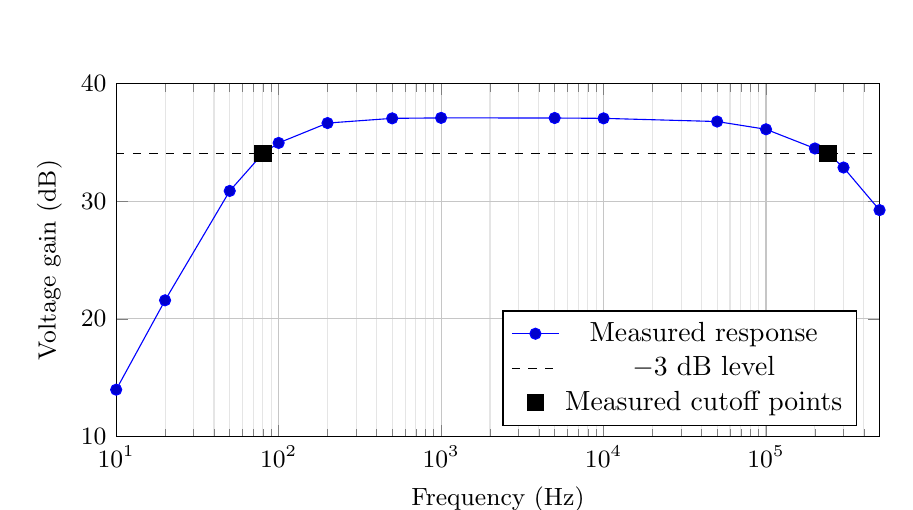
\begin{tikzpicture}
\begin{semilogxaxis}[
  width=0.93\textwidth,
  height=0.50\textwidth,
  xlabel={Frequency (\si{\hertz})},
  ylabel={Voltage gain (\si{\decibel})},
  xmin=10,
  xmax=500000,
  ymin=10,
  ymax=40,
  grid=both,
  minor grid style={gray!20},
  major grid style={gray!45},
  legend pos=south east,
  tick label style={font=\small},
  label style={font=\small},
]
\addplot+[mark=*] coordinates {
  (10,13.98)
  (20,21.58)
  (50,30.88)
  (80,34.07)
  (100,34.96)
  (200,36.65)
  (500,37.05)
  (1000,37.09)
  (5000,37.08)
  (10000,37.05)
  (50000,36.78)
  (100000,36.12)
  (200000,34.49)
  (240000,34.07)
  (300000,32.87)
  (500000,29.25)
};
\addlegendentry{Measured response}

\addplot[dashed,domain=10:500000,samples=2] {34.09};
\addlegendentry{$-3$ dB level}

\addplot[only marks,mark=square*,mark size=3pt]
coordinates {(80,34.07) (240000,34.07)};
\addlegendentry{Measured cutoff points}
\end{semilogxaxis}
\end{tikzpicture}
\caption{Illustrative measured frequency response of the RC-coupled amplifier.}
\label{fig:frequency-response}
\end{figure}

\begin{examplebox}
Figure~\ref{fig:frequency-response} shows an approximately constant gain in
the midband. The low-frequency reduction is caused by the finite reactances
of $C_1$, $C_2$, and $C_E$. The high-frequency reduction is associated with
transistor junction capacitances, the Miller effect, breadboard parasitic
capacitance, and oscilloscope-probe loading. The measured $-3$ dB
intersections occur near \SI{80}{\hertz} and
\SI{240}{\kilo\hertz}.
\end{examplebox}

% ============================================================
\section{Results and Discussion}
% ============================================================
\begin{sectionguide}
\begin{itemize}
  \item Begin with a concise summary of the principal findings.
  \item State whether the measurements support the design hypothesis and
        whether every specification was met.
  \item Compare theoretical, simulated, and measured values quantitatively.
  \item Refer directly to tables and figures as evidence.
  \item Explain discrepancies using component tolerance, transistor spread,
        source/load effects, probe capacitance, breadboard parasitics, noise,
        temperature, model limitations, and instrument uncertainty.
  \item Do not call every discrepancy ``human error.'' Give a testable
        circuit-level explanation.
  \item Do not introduce new results that were not presented in the Data,
        Observations, or Graphs sections.
  \item Discuss troubleshooting, repeatability, limitations, and technically
        justified improvements.
\end{itemize}
\end{sectionguide}

\begin{center}
\small
\begin{tabular}{lccccp{36mm}}
\toprule
Parameter & Theory & Simulation & Measurement & Error & Interpretation \\
\midrule
$V_{CE}$ &
\SI{6.45}{\volt} &
\SI{6.40}{\volt} &
\SI{6.35}{\volt} &
$1.55\%$ &
Active-region bias achieved \\

Midband gain &
\SI{84}{\volt\per\volt} &
\SI{76}{\volt\per\volt} &
\SI{71.5}{\volt\per\volt} &
$5.9\%$ vs.\ simulation &
Gain requirement satisfied \\

$f_L$ &
\SI{70}{\hertz} &
\SI{74}{\hertz} &
\SI{80}{\hertz} &
$8.1\%$ vs.\ simulation &
Capacitor tolerance and combined poles \\

$f_H$ &
--- &
\SI{260}{\kilo\hertz} &
\SI{240}{\kilo\hertz} &
$7.7\%$ vs.\ simulation &
Parasitic and probe capacitance \\

Bandwidth &
--- &
\SI{259.93}{\kilo\hertz} &
\SI{239.92}{\kilo\hertz} &
$7.7\%$ vs.\ simulation &
Broadband response obtained \\
\bottomrule
\end{tabular}
\end{center}

\begin{examplebox}
The measured DC operating point was
$V_{CE}=\SI{6.35}{\volt}$, close to the theoretical
\SI{6.45}{\volt}. This confirms that the transistor operated in the active
region and that the voltage-divider bias provided an appropriate quiescent
point.

The measured midband gain was
\SI{71.5}{\volt\per\volt}, compared with the simulated
\SI{76}{\volt\per\volt}. The measured value exceeded the stated requirement
of \SI{60}{\volt\per\volt}, so the gain specification was met. The remaining
difference is consistent with transistor-$\beta$ variation, finite output
resistance, nonzero emitter-bypass reactance, loading by the source and
oscilloscope, and resistor tolerance.

The measured lower cutoff frequency was approximately
\SI{80}{\hertz}, slightly above the simulated
\SI{74}{\hertz}. Electrolytic capacitors commonly have wider tolerance than
resistors, and the observed low-frequency response is the combined effect of
multiple poles rather than a single ideal pole.

The measured upper cutoff frequency was approximately
\SI{240}{\kilo\hertz}, below the simulated
\SI{260}{\kilo\hertz}. The likely causes are transistor junction-capacitance
variation, the Miller effect, breadboard wiring capacitance, and probe
capacitance that may not have been fully represented in the simulation.

The output phase reversal agreed with common-emitter theory. The small-signal
output remained approximately sinusoidal, while larger inputs caused
clipping as the transistor approached cutoff or saturation. Thus, the
experimental observations supported the design hypothesis within the
limitations of the components, model, and measurement setup.

A more rigorous follow-up could repeat the test using several transistor
samples, measure actual capacitor values, include probe capacitance in the
simulation, and construct the circuit on a PCB with shorter interconnections.
\end{examplebox}

\subsection*{11.1 Measurement uncertainty and limitations}

\begin{examplebox}
The reported results should be interpreted with the following limitations:
\begin{itemize}
  \item resistor and capacitor tolerance;
  \item unit-to-unit variation in BJT $\beta$, $V_{BE}$, and junction
        capacitances;
  \item oscilloscope amplitude accuracy, bandwidth, and probe capacitance;
  \item function-generator source resistance and frequency-dependent output;
  \item breadboard contact resistance and stray capacitance;
  \item finite reading resolution and possible temperature drift;
  \item differences between the simulator device model and the physical
        transistor.
\end{itemize}
Where a discrepancy changes the conclusion, estimate its uncertainty or
repeat the measurement rather than merely listing possible error sources.
\end{examplebox}

% ============================================================
\section{Conclusions}
% ============================================================
\begin{sectionguide}
\begin{itemize}
  \item Directly answer the objectives and the engineering challenge.
  \item State the most important measured numerical results.
  \item Clearly identify which specifications were or were not achieved.
  \item State what was learned about the circuit, design process, simulation,
        measurement, and evidence-based engineering judgment.
  \item Mention only improvements supported by the preceding analysis.
  \item Do not introduce new data or lengthy theory.
\end{itemize}
\end{sectionguide}

\begin{examplebox}
A voltage-divider-biased, single-stage RC-coupled common-emitter amplifier
was designed, simulated, constructed, and tested. The measured quiescent
collector-emitter voltage was \SI{6.35}{\volt}, confirming active-region
operation. The measured midband gain was approximately
\SI{71.5}{\volt\per\volt}, and the output was approximately
$180^\circ$ out of phase with the input. The lower and upper cutoff
frequencies were approximately \SI{80}{\hertz} and
\SI{240}{\kilo\hertz}, giving a bandwidth of approximately
\SI{239.92}{\kilo\hertz}.

The gain and lower-cutoff specifications were achieved. The measured results
were reasonably close to simulation, and the differences were consistent
with component tolerance, transistor parameter variation, loading, and
breadboard/probe parasitics. The experiment demonstrated the complete
engineering cycle of defining a problem, carrying out pre-lab design and
simulation, constructing and testing the circuit, analysing evidence,
explaining discrepancies, and communicating the outcome in a formal report.
\end{examplebox}

% ============================================================
\section{References}
% ============================================================
\begin{sectionguide}
\begin{itemize}
  \item List every source actually used: laboratory manual, textbooks,
        datasheets, simulator documentation, standards, and technical notes.
  \item Use a consistent engineering citation style, preferably IEEE style.
  \item Cite a source in the body wherever its equation, model, specification,
        figure, or design rule is used.
  \item Do not list sources that were not consulted.
\end{itemize}
\end{sectionguide}

\begin{thebibliography}{9}

\bibitem{sedra}
A. S. Sedra and K. C. Smith,
\textit{Microelectronic Circuits}, 8th ed.
New York, NY, USA: Oxford University Press, 2020.

\bibitem{boylestad}
R. L. Boylestad and L. Nashelsky,
\textit{Electronic Devices and Circuit Theory}, 11th ed.
Boston, MA, USA: Pearson, 2013.

\bibitem{bc547}
onsemi,
``BC546B, BC547A/B/C, BC548B/C NPN General-Purpose Transistors,''
BC547 series datasheet.

\bibitem{ltspice}
Analog Devices,
``LTspice Simulator Documentation,''
software documentation, accessed \today.

\bibitem{cetmanual}
Department of Electronics and Communication Engineering,
\textit{Analog Circuits Laboratory Manual},
College of Engineering Trivandrum, current academic year.

\bibitem{mitsmanual}
Muthoot Institute of Technology and Science,
\textit{Electronics Circuits Lab Manual},
laboratory instruction and technical-report guidance.

\end{thebibliography}

% ============================================================
% Optional report-support material
% ============================================================
\appendix

\section{Optional Appendix: Raw Data, Simulation, and Supporting Material}

Use appendices for material that supports verification but would interrupt
the main report:
\begin{itemize}
  \item complete unprocessed measurements and repeated trials;
  \item oscilloscope captures with scale, coupling, and probe information;
  \item SPICE netlist, model statement, and simulation settings;
  \item additional theoretical derivations;
  \item uncertainty calculations;
  \item measured component values and calibration information;
  \item photographs used to clarify breadboard layout or troubleshooting.
\end{itemize}

The main report should remain understandable without requiring the reader to
search through the appendices.

\section{Student Authorship and Team-Contribution Declaration}

Laboratory construction and data collection may be carried out as a team when
permitted by the instructor. However, the interpretation and written report
submitted under a student's name should be that student's own work, except
for properly acknowledged collaboration and cited sources.

\vspace{4mm}
\begin{tabularx}{\textwidth}{>{\bfseries}p{42mm} X}
Student's contribution &
\blankfield{105mm} \\[5mm]
Team members' contribution &
\blankfield{105mm} \\[5mm]
Shared data or resources used &
\blankfield{105mm} \\[5mm]
Student declaration &
I confirm that this report accurately records the work performed and that
the submitted analysis and writing comply with the course instructions. \\[5mm]
Student signature and date &
\blankfield{70mm}
\end{tabularx}

% ============================================================
% MUST REMAIN THE LAST SECTION
% ============================================================
\clearpage
\section{Instructor Evaluation}

\textit{This section is to be completed by the instructor or laboratory
evaluator. The assessment records preparation, experimental competence,
understanding, and continuous maintenance of the laboratory report/record.}

\vspace{3mm}

\begin{center}
\begin{tabularx}{\textwidth}{
  |>{\centering\arraybackslash}p{9mm}
  |>{\raggedright\arraybackslash}X
  |>{\centering\arraybackslash}p{23mm}
  |>{\centering\arraybackslash}p{25mm}|
}
\hline
\textbf{Sl. No.} &
\textbf{Evaluation Component and Indicators} &
\textbf{Maximum Marks} &
\textbf{Marks Awarded} \\
\hline

1 &
\textbf{Preparation / Pre-Lab Work}
\begin{itemize}[leftmargin=4mm,nosep]
  \item familiarity with the objective, theory, circuit, and procedure;
  \item completed design calculations and expected waveforms;
  \item completed simulation and prepared observation tables;
  \item component, pinout, rating, and safety checks.
\end{itemize}
&
\textbf{14}
&
\\
\hline

2 &
\textbf{In-Lab Experimental Performance}
\begin{itemize}[leftmargin=4mm,nosep]
  \item systematic circuit assembly and correct instrument connections;
  \item safe operation and proper use of power supply, DMM, function
        generator, and oscilloscope;
  \item accurate measurement and recording of data;
  \item logical troubleshooting and rechecking of anomalous readings;
  \item teamwork, care of equipment, and orderly completion of the experiment.
\end{itemize}
&
\textbf{14}
&
\\
\hline

3 &
\textbf{Viva Voce}
\begin{itemize}[leftmargin=4mm,nosep]
  \item understanding of circuit operation and design choices;
  \item ability to explain expected and measured waveforms;
  \item interpretation of gain, cutoff frequencies, bandwidth, biasing,
        loading, and sources of discrepancy.
\end{itemize}
&
\textbf{20}
&
\\
\hline

4 &
\textbf{Timely Completion of Lab Reports / Record
(Continuous Assessment)}
\begin{itemize}[leftmargin=4mm,nosep]
  \item regular and timely completion;
  \item complete observations, calculations, graphs, and results;
  \item comparison of theory, simulation, and experiment;
  \item clarity, organisation, technical accuracy, and neatness.
\end{itemize}
&
\textbf{12}
&
\\
\hline

\multicolumn{2}{|r|}{\textbf{Total}} &
\textbf{60} &
\\
\hline
\end{tabularx}
\end{center}

\vspace{6mm}

\begin{tabularx}{\textwidth}{>{\bfseries}p{45mm} X}
Instructor's remarks &
\blankfield{110mm} \\[7mm]
&
\blankfield{110mm} \\[7mm]
Performance grade &
\blankfield{55mm} \\[6mm]
Date &
\blankfield{45mm} \\[6mm]
Instructor's name and signature &
\blankfield{75mm}
\end{tabularx}

\end{document}
